% AUTO-GENERATED by writeup/make_rehaul_fi_pooled.py -- do not edit; re-run the script.
\providecommand{\ser}[2]{#2}\providecommand{\serx}[3]{#3}
\ifdefined\rhfipNOrigins\else% AUTO-GENERATED by writeup/make_rehaul_fi_pooled.py -- do not edit; re-run the script.
\providecommand{\ser}[2]{#2}\providecommand{\serx}[3]{#3}
% \rhfip... macros for writeup/rehaul/08_feature_importance.tex (results/tree_shap_w3000_2014start_fomcfix_2026-10-26, the
% FOMC-patched design, its linear reference inputs/fiw_gamma_fomcfix.npz; the window study's ...W... macros:
% results/fi_by_window_2014start_2026-10-22, pre-patch; the final pooled runs, W = 3,000 trading days).
\providecommand{\rhfipNOrigins}{}\renewcommand{\rhfipNOrigins}{126}  % monthly origins (re-estimations explained)
\providecommand{\rhfipNRows}{}\renewcommand{\rhfipNRows}{33{,}970}  % bars explained, every bar of the evaluation span
\providecommand{\rhfipOriginEvery}{}\renewcommand{\rhfipOriginEvery}{21}  % trading days between origins
\providecommand{\rhfipLastBlock}{}\renewcommand{\rhfipLastBlock}{18}  % trading days of the last origin's block
\providecommand{\rhfipFirstOrigin}{}\renewcommand{\rhfipFirstOrigin}{2~January~2014}  % first origin (10:00 bar)
\providecommand{\rhfipLastOrigin}{}\renewcommand{\rhfipLastOrigin}{5~April~2024}  % last origin
\providecommand{\rhfipLastDay}{}\renewcommand{\rhfipLastDay}{30~April~2024}  % day of the last bar explained
\providecommand{\rhfipWindowDays}{}\renewcommand{\rhfipWindowDays}{3{,}000}  % rolling window, trading days
\providecommand{\rhfipWindowBars}{}\renewcommand{\rhfipWindowBars}{39{,}000}  % rolling window, bars
\providecommand{\rhfipNCols}{}\renewcommand{\rhfipNCols}{564}  % predictors of the full set
\providecommand{\rhfipNGroups}{}\renewcommand{\rhfipNGroups}{48}  % predictor groups: 46 exogenous series + HAR components + calendar dummies
\providecommand{\rhfipNExog}{}\renewcommand{\rhfipNExog}{46}  % exogenous series
\providecommand{\rhfipNPerSeries}{}\renewcommand{\rhfipNPerSeries}{12}  % predictors per exogenous series: value and availability averages at six horizons
\providecommand{\rhfipNStd}{}\renewcommand{\rhfipNStd}{12}  % standard groups
\providecommand{\rhfipNNonStd}{}\renewcommand{\rhfipNNonStd}{36}  % non-standard series
\providecommand{\rhfipNStdExog}{}\renewcommand{\rhfipNStdExog}{10}  % standard exogenous series
\providecommand{\rhfipTuneLast}{}\renewcommand{\rhfipTuneLast}{31~December~2013}  % last day of the last tuning fold (fold 3)
\providecommand{\rhfipRidgePen}{}\renewcommand{\rhfipRidgePen}{\ensuremath{10^{3}}}
\providecommand{\rhfipLassoPen}{}\renewcommand{\rhfipLassoPen}{\ensuremath{10^{-4}}}
\providecommand{\rhfipEnetPen}{}\renewcommand{\rhfipEnetPen}{\ensuremath{10^{-3}}}
\providecommand{\rhfipHarPf}{}\renewcommand{\rhfipHarPf}{0.01}  % penalty factor, HAR block
\providecommand{\rhfipBootBlock}{}\renewcommand{\rhfipBootBlock}{12}  % bootstrap block, origins
\providecommand{\rhfipBootB}{}\renewcommand{\rhfipBootB}{2{,}000}
\providecommand{\rhfipCiLevel}{}\renewcommand{\rhfipCiLevel}{95}  % percentile intervals of both rules (RULE_shap.txt, RULE_fiw.txt)
\providecommand{\rhfipShapeMin}{}\renewcommand{\rhfipShapeMin}{0.5}  % M3 selection: share of at least this many percent
\providecommand{\rhfipTopN}{}\renewcommand{\rhfipTopN}{10}  % length of the top lists compared (m2_rank.csv top10_overlap)
\providecommand{\rhfipSlopeUnit}{}\renewcommand{\rhfipSlopeUnit}{1{,}000}  % trading days per unit of the window slope
\providecommand{\rhfipNMom}{}\renewcommand{\rhfipNMom}{seven}  % the futures' realized moments (standard)
\providecommand{\rhfipLgbmGateEq}{}\renewcommand{\rhfipLgbmGateEq}{126}  % origins bit-equal to the merged every-bar walk
\providecommand{\rhfipXgbGateEq}{}\renewcommand{\rhfipXgbGateEq}{126}  % origins bit-equal to the merged every-bar walk
\providecommand{\rhfipRfGateEq}{}\renewcommand{\rhfipRfGateEq}{126}  % origins bit-equal to the merged every-bar walk
\providecommand{\rhfipRfGateAtShap}{}\renewcommand{\rhfipRfGateAtShap}{126}  % forest origins the walk had written when the SHAP gate ran
\providecommand{\rhfipXgbAddMax}{}\renewcommand{\rhfipXgbAddMax}{\ensuremath{3.7\times 10^{-6}}}  % XGBoost additivity, float32
\providecommand{\rhfipXgbAddTol}{}\renewcommand{\rhfipXgbAddTol}{\ensuremath{10^{-5}}}
\providecommand{\rhfipAddMaxDouble}{}\renewcommand{\rhfipAddMaxDouble}{\ensuremath{5.1\times 10^{-14}}}
\providecommand{\rhfipLinGateMax}{}\renewcommand{\rhfipLinGateMax}{\ensuremath{4.4\times 10^{-16}}}  % linear replay vs walk forecasts, W = 3,000
\providecommand{\rhfipInterRows}{}\renewcommand{\rhfipInterRows}{1{,}008}  % M5 rows
\providecommand{\rhfipInterPerOrigin}{}\renewcommand{\rhfipInterPerOrigin}{8}  % M5 rows per origin
\providecommand{\rhfipFomcRows}{}\renewcommand{\rhfipFomcRows}{1{,}014}
\providecommand{\rhfipFomcDaysShap}{}\renewcommand{\rhfipFomcDaysShap}{78}  % FOMC statement days in the SHAP subset (M4; releases.parquet only)
\providecommand{\rhfipFomcDays}{}\renewcommand{\rhfipFomcDays}{81}  % scheduled FOMC statement days in the span (loader calendar)
\providecommand{\rhfipFomcDaysMissing}{}\renewcommand{\rhfipFomcDaysMissing}{3}  % statement days the SHAP subset leaves out (counted with the other days; the patched rerun's reducer keeps releases.parquet's days)
\providecommand{\rhfipNHolSessions}{}\renewcommand{\rhfipNHolSessions}{64}  % NYSE-holiday futures sessions among the explained bars (not scored in Table 1)
\providecommand{\rhfipNHolBars}{}\renewcommand{\rhfipNHolBars}{443}  % their regular-hours bars
\providecommand{\rhfipVixLo}{}\renewcommand{\rhfipVixLo}{13.96}
\providecommand{\rhfipVixHi}{}\renewcommand{\rhfipVixHi}{19.02}
\providecommand{\rhfipLgbmHar}{}\renewcommand{\rhfipLgbmHar}{51.7}
\providecommand{\rhfipLgbmHarLo}{}\renewcommand{\rhfipLgbmHarLo}{49.5}
\providecommand{\rhfipLgbmHarHi}{}\renewcommand{\rhfipLgbmHarHi}{53.7}
\providecommand{\rhfipLgbmMom}{}\renewcommand{\rhfipLgbmMom}{22.3}
\providecommand{\rhfipLgbmNs}{}\renewcommand{\rhfipLgbmNs}{21.8}
\providecommand{\rhfipLgbmNsLo}{}\renewcommand{\rhfipLgbmNsLo}{20.4}
\providecommand{\rhfipLgbmNsHi}{}\renewcommand{\rhfipLgbmNsHi}{23.4}
\providecommand{\rhfipLgbmNsEx}{}\renewcommand{\rhfipLgbmNsEx}{45.9}
\providecommand{\rhfipLgbmNsExLo}{}\renewcommand{\rhfipLgbmNsExLo}{44.2}
\providecommand{\rhfipLgbmNsExHi}{}\renewcommand{\rhfipLgbmNsExHi}{47.7}
\providecommand{\rhfipXgbHar}{}\renewcommand{\rhfipXgbHar}{52.0}
\providecommand{\rhfipXgbHarLo}{}\renewcommand{\rhfipXgbHarLo}{50.0}
\providecommand{\rhfipXgbHarHi}{}\renewcommand{\rhfipXgbHarHi}{53.8}
\providecommand{\rhfipXgbMom}{}\renewcommand{\rhfipXgbMom}{23.6}
\providecommand{\rhfipXgbNs}{}\renewcommand{\rhfipXgbNs}{20.6}
\providecommand{\rhfipXgbNsLo}{}\renewcommand{\rhfipXgbNsLo}{19.2}
\providecommand{\rhfipXgbNsHi}{}\renewcommand{\rhfipXgbNsHi}{22.2}
\providecommand{\rhfipXgbNsEx}{}\renewcommand{\rhfipXgbNsEx}{43.6}
\providecommand{\rhfipXgbNsExLo}{}\renewcommand{\rhfipXgbNsExLo}{41.8}
\providecommand{\rhfipXgbNsExHi}{}\renewcommand{\rhfipXgbNsExHi}{45.7}
\providecommand{\rhfipRfHar}{}\renewcommand{\rhfipRfHar}{57.6}
\providecommand{\rhfipRfHarLo}{}\renewcommand{\rhfipRfHarLo}{55.4}
\providecommand{\rhfipRfHarHi}{}\renewcommand{\rhfipRfHarHi}{59.6}
\providecommand{\rhfipRfMom}{}\renewcommand{\rhfipRfMom}{20.7}
\providecommand{\rhfipRfNs}{}\renewcommand{\rhfipRfNs}{18.6}
\providecommand{\rhfipRfNsLo}{}\renewcommand{\rhfipRfNsLo}{17.2}
\providecommand{\rhfipRfNsHi}{}\renewcommand{\rhfipRfNsHi}{20.3}
\providecommand{\rhfipRfNsEx}{}\renewcommand{\rhfipRfNsEx}{44.2}
\providecommand{\rhfipRfNsExLo}{}\renewcommand{\rhfipRfNsExLo}{42.1}
\providecommand{\rhfipRfNsExHi}{}\renewcommand{\rhfipRfNsExHi}{46.5}
\providecommand{\rhfipRidgeNsEx}{}\renewcommand{\rhfipRidgeNsEx}{68.8}
\providecommand{\rhfipRidgeNs}{}\renewcommand{\rhfipRidgeNs}{55.6}
\providecommand{\rhfipRidgeHar}{}\renewcommand{\rhfipRidgeHar}{17.5}
\providecommand{\rhfipLassoNsEx}{}\renewcommand{\rhfipLassoNsEx}{82.5}
\providecommand{\rhfipLassoNs}{}\renewcommand{\rhfipLassoNs}{76.5}
\providecommand{\rhfipLassoHar}{}\renewcommand{\rhfipLassoHar}{6.7}
\providecommand{\rhfipEnetNsEx}{}\renewcommand{\rhfipEnetNsEx}{60.0}
\providecommand{\rhfipEnetNs}{}\renewcommand{\rhfipEnetNs}{42.9}
\providecommand{\rhfipEnetHar}{}\renewcommand{\rhfipEnetHar}{26.4}
\providecommand{\rhfipHarMin}{}\renewcommand{\rhfipHarMin}{51.7}
\providecommand{\rhfipHarMax}{}\renewcommand{\rhfipHarMax}{57.6}
\providecommand{\rhfipMomMin}{}\renewcommand{\rhfipMomMin}{20.7}
\providecommand{\rhfipMomMax}{}\renewcommand{\rhfipMomMax}{23.6}
\providecommand{\rhfipNsExMin}{}\renewcommand{\rhfipNsExMin}{43.6}
\providecommand{\rhfipNsExMax}{}\renewcommand{\rhfipNsExMax}{45.9}
\providecommand{\rhfipSentMin}{}\renewcommand{\rhfipSentMin}{0.6}
\providecommand{\rhfipSentMax}{}\renewcommand{\rhfipSentMax}{0.8}
\providecommand{\rhfipVdMin}{}\renewcommand{\rhfipVdMin}{0.2}
\providecommand{\rhfipVdMax}{}\renewcommand{\rhfipVdMax}{0.3}
\providecommand{\rhfipFomcBucketMin}{}\renewcommand{\rhfipFomcBucketMin}{1.4}
\providecommand{\rhfipFomcBucketMax}{}\renewcommand{\rhfipFomcBucketMax}{2.3}
\providecommand{\rhfipVvixMin}{}\renewcommand{\rhfipVvixMin}{0.2}
\providecommand{\rhfipVvixMax}{}\renewcommand{\rhfipVvixMax}{0.3}
\providecommand{\rhfipVixThreeMMin}{}\renewcommand{\rhfipVixThreeMMin}{0.3}
\providecommand{\rhfipVixThreeMMax}{}\renewcommand{\rhfipVixThreeMMax}{0.7}
\providecommand{\rhfipFomcDayMin}{}\renewcommand{\rhfipFomcDayMin}{0.1}
\providecommand{\rhfipFomcDayMax}{}\renewcommand{\rhfipFomcDayMax}{0.1}
\providecommand{\rhfipNsOne}{}\renewcommand{\rhfipNsOne}{\ensuremath{\ser{sumabsret_vwstock}{\mathrm{RAV}^{\mathrm{VW}}}}}
\providecommand{\rhfipNsOneMin}{}\renewcommand{\rhfipNsOneMin}{2.4}
\providecommand{\rhfipNsOneMax}{}\renewcommand{\rhfipNsOneMax}{3.9}
\providecommand{\rhfipNsOneLgbm}{}\renewcommand{\rhfipNsOneLgbm}{3.5}
\providecommand{\rhfipNsOneXgb}{}\renewcommand{\rhfipNsOneXgb}{3.9}
\providecommand{\rhfipNsOneRf}{}\renewcommand{\rhfipNsOneRf}{2.4}
\providecommand{\rhfipNsTwo}{}\renewcommand{\rhfipNsTwo}{\ensuremath{\ser{sumabsret_ewstock}{\mathrm{RAV}^{\mathrm{EW}}}}}
\providecommand{\rhfipNsTwoMin}{}\renewcommand{\rhfipNsTwoMin}{1.9}
\providecommand{\rhfipNsTwoMax}{}\renewcommand{\rhfipNsTwoMax}{3.9}
\providecommand{\rhfipNsTwoLgbm}{}\renewcommand{\rhfipNsTwoLgbm}{3.9}
\providecommand{\rhfipNsTwoXgb}{}\renewcommand{\rhfipNsTwoXgb}{3.8}
\providecommand{\rhfipNsTwoRf}{}\renewcommand{\rhfipNsTwoRf}{1.9}
\providecommand{\rhfipNsThree}{}\renewcommand{\rhfipNsThree}{\ensuremath{\ser{fomc_until_inv}{\mathrm{FOMC}^{\mathrm{next}}}}}
\providecommand{\rhfipNsThreeMin}{}\renewcommand{\rhfipNsThreeMin}{1.1}
\providecommand{\rhfipNsThreeMax}{}\renewcommand{\rhfipNsThreeMax}{2.0}
\providecommand{\rhfipNsThreeLgbm}{}\renewcommand{\rhfipNsThreeLgbm}{2.0}
\providecommand{\rhfipNsThreeXgb}{}\renewcommand{\rhfipNsThreeXgb}{2.0}
\providecommand{\rhfipNsThreeRf}{}\renewcommand{\rhfipNsThreeRf}{1.1}
\providecommand{\rhfipNsFour}{}\renewcommand{\rhfipNsFour}{\ensuremath{\ser{ofi_vwstock}{\mathrm{OFI}^{\mathrm{VW}}}}}
\providecommand{\rhfipNsFourMin}{}\renewcommand{\rhfipNsFourMin}{1.4}
\providecommand{\rhfipNsFourMax}{}\renewcommand{\rhfipNsFourMax}{1.8}
\providecommand{\rhfipNsFourLgbm}{}\renewcommand{\rhfipNsFourLgbm}{1.8}
\providecommand{\rhfipNsFourXgb}{}\renewcommand{\rhfipNsFourXgb}{1.7}
\providecommand{\rhfipNsFourRf}{}\renewcommand{\rhfipNsFourRf}{1.4}
\providecommand{\rhfipNsFive}{}\renewcommand{\rhfipNsFive}{\ensuremath{\ser{effspread_vwstock}{\mathrm{EffSpread}^{\mathrm{VW}}}}}
\providecommand{\rhfipNsFiveMin}{}\renewcommand{\rhfipNsFiveMin}{1.2}
\providecommand{\rhfipNsFiveMax}{}\renewcommand{\rhfipNsFiveMax}{1.3}
\providecommand{\rhfipNsFiveLgbm}{}\renewcommand{\rhfipNsFiveLgbm}{1.2}
\providecommand{\rhfipNsFiveXgb}{}\renewcommand{\rhfipNsFiveXgb}{1.2}
\providecommand{\rhfipNsFiveRf}{}\renewcommand{\rhfipNsFiveRf}{1.3}
\providecommand{\rhfipTreeTopOne}{}\renewcommand{\rhfipTreeTopOne}{\ensuremath{\ser{sumabsret}{\mathrm{RAV}}}}
\providecommand{\rhfipTreeTopTwo}{}\renewcommand{\rhfipTreeTopTwo}{\ensuremath{\ser{sumret}{r}}}
\providecommand{\rhfipLgbmTopOneEx}{}\renewcommand{\rhfipLgbmTopOneEx}{20.3}
\providecommand{\rhfipXgbTopOneEx}{}\renewcommand{\rhfipXgbTopOneEx}{24.7}
\providecommand{\rhfipRfTopOneEx}{}\renewcommand{\rhfipRfTopOneEx}{29.2}
\providecommand{\rhfipRidgeTopOne}{}\renewcommand{\rhfipRidgeTopOne}{\ensuremath{\ser{fomc_until_inv}{\mathrm{FOMC}^{\mathrm{next}}}}}
\providecommand{\rhfipRidgeTopOneEx}{}\renewcommand{\rhfipRidgeTopOneEx}{9.0}
\providecommand{\rhfipLgbmNUsedAll}{}\renewcommand{\rhfipLgbmNUsedAll}{42}  % exogenous series split on at every origin
\providecommand{\rhfipLgbmUsedMin}{}\renewcommand{\rhfipLgbmUsedMin}{58}
\providecommand{\rhfipXgbNUsedAll}{}\renewcommand{\rhfipXgbNUsedAll}{43}  % exogenous series split on at every origin
\providecommand{\rhfipXgbUsedMin}{}\renewcommand{\rhfipXgbUsedMin}{72}
\providecommand{\rhfipRfNUsedAll}{}\renewcommand{\rhfipRfNUsedAll}{46}  % exogenous series split on at every origin
\providecommand{\rhfipRfUsedMin}{}\renewcommand{\rhfipRfUsedMin}{126}
\providecommand{\rhfipLgbmDRidge}{}\renewcommand{\rhfipLgbmDRidge}{\ensuremath{-}22.9}
\providecommand{\rhfipLgbmDRidgeLo}{}\renewcommand{\rhfipLgbmDRidgeLo}{\ensuremath{-}24.8}
\providecommand{\rhfipLgbmDRidgeHi}{}\renewcommand{\rhfipLgbmDRidgeHi}{\ensuremath{-}21.1}
\providecommand{\rhfipLgbmDLasso}{}\renewcommand{\rhfipLgbmDLasso}{\ensuremath{-}36.6}
\providecommand{\rhfipLgbmDLassoLo}{}\renewcommand{\rhfipLgbmDLassoLo}{\ensuremath{-}39.1}
\providecommand{\rhfipLgbmDLassoHi}{}\renewcommand{\rhfipLgbmDLassoHi}{\ensuremath{-}34.4}
\providecommand{\rhfipLgbmDEnet}{}\renewcommand{\rhfipLgbmDEnet}{\ensuremath{-}14.1}
\providecommand{\rhfipLgbmDEnetLo}{}\renewcommand{\rhfipLgbmDEnetLo}{\ensuremath{-}15.7}
\providecommand{\rhfipLgbmDEnetHi}{}\renewcommand{\rhfipLgbmDEnetHi}{\ensuremath{-}12.7}
\providecommand{\rhfipXgbDRidge}{}\renewcommand{\rhfipXgbDRidge}{\ensuremath{-}25.1}
\providecommand{\rhfipXgbDRidgeLo}{}\renewcommand{\rhfipXgbDRidgeLo}{\ensuremath{-}27.0}
\providecommand{\rhfipXgbDRidgeHi}{}\renewcommand{\rhfipXgbDRidgeHi}{\ensuremath{-}23.3}
\providecommand{\rhfipXgbDLasso}{}\renewcommand{\rhfipXgbDLasso}{\ensuremath{-}38.9}
\providecommand{\rhfipXgbDLassoLo}{}\renewcommand{\rhfipXgbDLassoLo}{\ensuremath{-}41.4}
\providecommand{\rhfipXgbDLassoHi}{}\renewcommand{\rhfipXgbDLassoHi}{\ensuremath{-}36.6}
\providecommand{\rhfipXgbDEnet}{}\renewcommand{\rhfipXgbDEnet}{\ensuremath{-}16.3}
\providecommand{\rhfipXgbDEnetLo}{}\renewcommand{\rhfipXgbDEnetLo}{\ensuremath{-}17.8}
\providecommand{\rhfipXgbDEnetHi}{}\renewcommand{\rhfipXgbDEnetHi}{\ensuremath{-}14.9}
\providecommand{\rhfipRfDRidge}{}\renewcommand{\rhfipRfDRidge}{\ensuremath{-}24.5}
\providecommand{\rhfipRfDRidgeLo}{}\renewcommand{\rhfipRfDRidgeLo}{\ensuremath{-}26.3}
\providecommand{\rhfipRfDRidgeHi}{}\renewcommand{\rhfipRfDRidgeHi}{\ensuremath{-}22.9}
\providecommand{\rhfipRfDLasso}{}\renewcommand{\rhfipRfDLasso}{\ensuremath{-}38.3}
\providecommand{\rhfipRfDLassoLo}{}\renewcommand{\rhfipRfDLassoLo}{\ensuremath{-}40.5}
\providecommand{\rhfipRfDLassoHi}{}\renewcommand{\rhfipRfDLassoHi}{\ensuremath{-}36.3}
\providecommand{\rhfipRfDEnet}{}\renewcommand{\rhfipRfDEnet}{\ensuremath{-}15.7}
\providecommand{\rhfipRfDEnetLo}{}\renewcommand{\rhfipRfDEnetLo}{\ensuremath{-}17.0}
\providecommand{\rhfipRfDEnetHi}{}\renewcommand{\rhfipRfDEnetHi}{\ensuremath{-}14.4}
\providecommand{\rhfipNDLess}{}\renewcommand{\rhfipNDLess}{27}  % tree-minus-linear D with the 95% interval below 0
\providecommand{\rhfipNDAll}{}\renewcommand{\rhfipNDAll}{27}  % D comparisons: 3 trees x 3 linear models x 3 denominators
\providecommand{\rhfipLgbmSpRidge}{}\renewcommand{\rhfipLgbmSpRidge}{0.57}
\providecommand{\rhfipLgbmTopRidge}{}\renewcommand{\rhfipLgbmTopRidge}{6}
\providecommand{\rhfipLgbmSpLasso}{}\renewcommand{\rhfipLgbmSpLasso}{0.49}
\providecommand{\rhfipLgbmTopLasso}{}\renewcommand{\rhfipLgbmTopLasso}{5}
\providecommand{\rhfipLgbmSpEnet}{}\renewcommand{\rhfipLgbmSpEnet}{0.66}
\providecommand{\rhfipLgbmTopEnet}{}\renewcommand{\rhfipLgbmTopEnet}{6}
\providecommand{\rhfipXgbSpRidge}{}\renewcommand{\rhfipXgbSpRidge}{0.55}
\providecommand{\rhfipXgbTopRidge}{}\renewcommand{\rhfipXgbTopRidge}{6}
\providecommand{\rhfipXgbSpLasso}{}\renewcommand{\rhfipXgbSpLasso}{0.47}
\providecommand{\rhfipXgbTopLasso}{}\renewcommand{\rhfipXgbTopLasso}{5}
\providecommand{\rhfipXgbSpEnet}{}\renewcommand{\rhfipXgbSpEnet}{0.63}
\providecommand{\rhfipXgbTopEnet}{}\renewcommand{\rhfipXgbTopEnet}{6}
\providecommand{\rhfipRfSpRidge}{}\renewcommand{\rhfipRfSpRidge}{0.53}
\providecommand{\rhfipRfTopRidge}{}\renewcommand{\rhfipRfTopRidge}{5}
\providecommand{\rhfipRfSpLasso}{}\renewcommand{\rhfipRfSpLasso}{0.43}
\providecommand{\rhfipRfTopLasso}{}\renewcommand{\rhfipRfTopLasso}{4}
\providecommand{\rhfipRfSpEnet}{}\renewcommand{\rhfipRfSpEnet}{0.60}
\providecommand{\rhfipRfTopEnet}{}\renewcommand{\rhfipRfTopEnet}{5}
\providecommand{\rhfipSpLgbmXgb}{}\renewcommand{\rhfipSpLgbmXgb}{0.99}
\providecommand{\rhfipSpLgbmRf}{}\renewcommand{\rhfipSpLgbmRf}{0.90}
\providecommand{\rhfipSpXgbRf}{}\renewcommand{\rhfipSpXgbRf}{0.89}
\providecommand{\rhfipRidgeRankFomcUntil}{}\renewcommand{\rhfipRidgeRankFomcUntil}{1}
\providecommand{\rhfipTreeRankFomcUntilMin}{}\renewcommand{\rhfipTreeRankFomcUntilMin}{6}
\providecommand{\rhfipTreeRankFomcUntilMax}{}\renewcommand{\rhfipTreeRankFomcUntilMax}{10}
\providecommand{\rhfipRidgeRankFomcDay}{}\renewcommand{\rhfipRidgeRankFomcDay}{9}
\providecommand{\rhfipTreeRankFomcDayMin}{}\renewcommand{\rhfipTreeRankFomcDayMin}{39}
\providecommand{\rhfipTreeRankFomcDayMax}{}\renewcommand{\rhfipTreeRankFomcDayMax}{43}
\providecommand{\rhfipFomcUntil}{}\renewcommand{\rhfipFomcUntil}{\ensuremath{\ser{fomc_until_inv}{\mathrm{FOMC}^{\mathrm{next}}}}}
\providecommand{\rhfipFomcDay}{}\renewcommand{\rhfipFomcDay}{\ensuremath{\ser{fomc_day}{\mathrm{FOMC}^{\mathrm{day}}}}}
\providecommand{\rhfipAbsVw}{}\renewcommand{\rhfipAbsVw}{\ensuremath{\ser{sumabsret_vwstock}{\mathrm{RAV}^{\mathrm{VW}}}}}
\providecommand{\rhfipOfi}{}\renewcommand{\rhfipOfi}{\ensuremath{\ser{ofi_vwstock}{\mathrm{OFI}^{\mathrm{VW}}}}}
\providecommand{\rhfipLgbmNeff}{}\renewcommand{\rhfipLgbmNeff}{11.0}
\providecommand{\rhfipLgbmNHalf}{}\renewcommand{\rhfipLgbmNHalf}{4}
\providecommand{\rhfipLgbmNEighty}{}\renewcommand{\rhfipLgbmNEighty}{13}
\providecommand{\rhfipXgbNeff}{}\renewcommand{\rhfipXgbNeff}{9.1}
\providecommand{\rhfipXgbNHalf}{}\renewcommand{\rhfipXgbNHalf}{4}
\providecommand{\rhfipXgbNEighty}{}\renewcommand{\rhfipXgbNEighty}{11}
\providecommand{\rhfipRfNeff}{}\renewcommand{\rhfipRfNeff}{8.9}
\providecommand{\rhfipRfNHalf}{}\renewcommand{\rhfipRfNHalf}{4}
\providecommand{\rhfipRfNEighty}{}\renewcommand{\rhfipRfNEighty}{16}
\providecommand{\rhfipRidgeNeff}{}\renewcommand{\rhfipRidgeNeff}{28.5}
\providecommand{\rhfipRidgeNHalf}{}\renewcommand{\rhfipRidgeNHalf}{11}
\providecommand{\rhfipRidgeNEighty}{}\renewcommand{\rhfipRidgeNEighty}{26}
\providecommand{\rhfipLassoNeff}{}\renewcommand{\rhfipLassoNeff}{5.1}
\providecommand{\rhfipLassoNHalf}{}\renewcommand{\rhfipLassoNHalf}{2}
\providecommand{\rhfipLassoNEighty}{}\renewcommand{\rhfipLassoNEighty}{11}
\providecommand{\rhfipEnetNeff}{}\renewcommand{\rhfipEnetNeff}{16.2}
\providecommand{\rhfipEnetNHalf}{}\renewcommand{\rhfipEnetNHalf}{6}
\providecommand{\rhfipEnetNEighty}{}\renewcommand{\rhfipEnetNEighty}{15}
\providecommand{\rhfipYearFirst}{}\renewcommand{\rhfipYearFirst}{2014}
\providecommand{\rhfipYearLast}{}\renewcommand{\rhfipYearLast}{2024}
\providecommand{\rhfipLgbmNsYearMin}{}\renewcommand{\rhfipLgbmNsYearMin}{18.1}
\providecommand{\rhfipLgbmNsYearMinYr}{}\renewcommand{\rhfipLgbmNsYearMinYr}{2021}
\providecommand{\rhfipLgbmNsYearMax}{}\renewcommand{\rhfipLgbmNsYearMax}{25.6}
\providecommand{\rhfipLgbmNsYearMaxYr}{}\renewcommand{\rhfipLgbmNsYearMaxYr}{2015}
\providecommand{\rhfipLgbmHarYearMax}{}\renewcommand{\rhfipLgbmHarYearMax}{57.4}
\providecommand{\rhfipLgbmHarYearMaxYr}{}\renewcommand{\rhfipLgbmHarYearMaxYr}{2021}
\providecommand{\rhfipLgbmHarYearMin}{}\renewcommand{\rhfipLgbmHarYearMin}{44.6}
\providecommand{\rhfipLgbmHarYearMinYr}{}\renewcommand{\rhfipLgbmHarYearMinYr}{2017}
\providecommand{\rhfipXgbNsYearMin}{}\renewcommand{\rhfipXgbNsYearMin}{17.2}
\providecommand{\rhfipXgbNsYearMinYr}{}\renewcommand{\rhfipXgbNsYearMinYr}{2021}
\providecommand{\rhfipXgbNsYearMax}{}\renewcommand{\rhfipXgbNsYearMax}{24.3}
\providecommand{\rhfipXgbNsYearMaxYr}{}\renewcommand{\rhfipXgbNsYearMaxYr}{2015}
\providecommand{\rhfipXgbHarYearMax}{}\renewcommand{\rhfipXgbHarYearMax}{57.0}
\providecommand{\rhfipXgbHarYearMaxYr}{}\renewcommand{\rhfipXgbHarYearMaxYr}{2021}
\providecommand{\rhfipXgbHarYearMin}{}\renewcommand{\rhfipXgbHarYearMin}{45.8}
\providecommand{\rhfipXgbHarYearMinYr}{}\renewcommand{\rhfipXgbHarYearMinYr}{2017}
\providecommand{\rhfipRfNsYearMin}{}\renewcommand{\rhfipRfNsYearMin}{15.2}
\providecommand{\rhfipRfNsYearMinYr}{}\renewcommand{\rhfipRfNsYearMinYr}{2021}
\providecommand{\rhfipRfNsYearMax}{}\renewcommand{\rhfipRfNsYearMax}{22.9}
\providecommand{\rhfipRfNsYearMaxYr}{}\renewcommand{\rhfipRfNsYearMaxYr}{2015}
\providecommand{\rhfipRfHarYearMax}{}\renewcommand{\rhfipRfHarYearMax}{62.3}
\providecommand{\rhfipRfHarYearMaxYr}{}\renewcommand{\rhfipRfHarYearMaxYr}{2019}
\providecommand{\rhfipRfHarYearMin}{}\renewcommand{\rhfipRfHarYearMin}{50.4}
\providecommand{\rhfipRfHarYearMinYr}{}\renewcommand{\rhfipRfHarYearMinYr}{2017}
\providecommand{\rhfipNsYearMinYr}{}\renewcommand{\rhfipNsYearMinYr}{2021}  % the year of every tree's lowest non-standard share
\providecommand{\rhfipDipFirst}{}\renewcommand{\rhfipDipFirst}{2018}  % first of the years in which every tree's non-standard share is below its pooled share
\providecommand{\rhfipDipLast}{}\renewcommand{\rhfipDipLast}{2022}
\providecommand{\rhfipRidgeNsExYearMin}{}\renewcommand{\rhfipRidgeNsExYearMin}{65.1}
\providecommand{\rhfipRidgeNsExYearMinYr}{}\renewcommand{\rhfipRidgeNsExYearMinYr}{2021}
\providecommand{\rhfipRidgeNsExYearMax}{}\renewcommand{\rhfipRidgeNsExYearMax}{72.4}
\providecommand{\rhfipRidgeNsExYearMaxYr}{}\renewcommand{\rhfipRidgeNsExYearMaxYr}{2017}
\providecommand{\rhfipLassoNsExYearMin}{}\renewcommand{\rhfipLassoNsExYearMin}{77.1}
\providecommand{\rhfipLassoNsExYearMinYr}{}\renewcommand{\rhfipLassoNsExYearMinYr}{2021}
\providecommand{\rhfipLassoNsExYearMax}{}\renewcommand{\rhfipLassoNsExYearMax}{87.1}
\providecommand{\rhfipLassoNsExYearMaxYr}{}\renewcommand{\rhfipLassoNsExYearMaxYr}{2017}
\providecommand{\rhfipEnetNsExYearMin}{}\renewcommand{\rhfipEnetNsExYearMin}{56.1}
\providecommand{\rhfipEnetNsExYearMinYr}{}\renewcommand{\rhfipEnetNsExYearMinYr}{2019}
\providecommand{\rhfipEnetNsExYearMax}{}\renewcommand{\rhfipEnetNsExYearMax}{65.2}
\providecommand{\rhfipEnetNsExYearMaxYr}{}\renewcommand{\rhfipEnetNsExYearMaxYr}{2014}
\providecommand{\rhfipLgbmNsExYearMin}{}\renewcommand{\rhfipLgbmNsExYearMin}{42.3}
\providecommand{\rhfipLgbmNsExYearMax}{}\renewcommand{\rhfipLgbmNsExYearMax}{50.1}
\providecommand{\rhfipXgbNsExYearMin}{}\renewcommand{\rhfipXgbNsExYearMin}{39.4}
\providecommand{\rhfipXgbNsExYearMax}{}\renewcommand{\rhfipXgbNsExYearMax}{48.9}
\providecommand{\rhfipRfNsExYearMin}{}\renewcommand{\rhfipRfNsExYearMin}{39.5}
\providecommand{\rhfipRfNsExYearMax}{}\renewcommand{\rhfipRfNsExYearMax}{50.9}
\providecommand{\rhfipLgbmNShape}{}\renewcommand{\rhfipLgbmNShape}{11}  % non-standard series at >= 0.5% (M3)
\providecommand{\rhfipLgbmNMono}{}\renewcommand{\rhfipLgbmNMono}{7}
\providecommand{\rhfipLgbmNIrr}{}\renewcommand{\rhfipLgbmNIrr}{3}
\providecommand{\rhfipLgbmNStep}{}\renewcommand{\rhfipLgbmNStep}{1}
\providecommand{\rhfipLgbmNFlat}{}\renewcommand{\rhfipLgbmNFlat}{0}
\providecommand{\rhfipLgbmNThresh}{}\renewcommand{\rhfipLgbmNThresh}{0}
\providecommand{\rhfipLgbmNU}{}\renewcommand{\rhfipLgbmNU}{0}
\providecommand{\rhfipLgbmNAsym}{}\renewcommand{\rhfipLgbmNAsym}{9}
\providecommand{\rhfipXgbNShape}{}\renewcommand{\rhfipXgbNShape}{10}  % non-standard series at >= 0.5% (M3)
\providecommand{\rhfipXgbNMono}{}\renewcommand{\rhfipXgbNMono}{5}
\providecommand{\rhfipXgbNIrr}{}\renewcommand{\rhfipXgbNIrr}{3}
\providecommand{\rhfipXgbNStep}{}\renewcommand{\rhfipXgbNStep}{0}
\providecommand{\rhfipXgbNFlat}{}\renewcommand{\rhfipXgbNFlat}{1}
\providecommand{\rhfipXgbNThresh}{}\renewcommand{\rhfipXgbNThresh}{1}
\providecommand{\rhfipXgbNU}{}\renewcommand{\rhfipXgbNU}{0}
\providecommand{\rhfipXgbNAsym}{}\renewcommand{\rhfipXgbNAsym}{8}
\providecommand{\rhfipRfNShape}{}\renewcommand{\rhfipRfNShape}{13}  % non-standard series at >= 0.5% (M3)
\providecommand{\rhfipRfNMono}{}\renewcommand{\rhfipRfNMono}{10}
\providecommand{\rhfipRfNIrr}{}\renewcommand{\rhfipRfNIrr}{3}
\providecommand{\rhfipRfNStep}{}\renewcommand{\rhfipRfNStep}{0}
\providecommand{\rhfipRfNFlat}{}\renewcommand{\rhfipRfNFlat}{0}
\providecommand{\rhfipRfNThresh}{}\renewcommand{\rhfipRfNThresh}{0}
\providecommand{\rhfipRfNU}{}\renewcommand{\rhfipRfNU}{0}
\providecommand{\rhfipRfNAsym}{}\renewcommand{\rhfipRfNAsym}{13}
\providecommand{\rhfipNUThreshAll}{}\renewcommand{\rhfipNUThreshAll}{1}  % U-shaped, inverted-U or threshold profiles in any tree
\providecommand{\rhfipAbsVwLgbmLo}{}\renewcommand{\rhfipAbsVwLgbmLo}{\ensuremath{-}1.4}
\providecommand{\rhfipAbsVwLgbmHi}{}\renewcommand{\rhfipAbsVwLgbmHi}{3.9}
\providecommand{\rhfipAbsVwXgbLo}{}\renewcommand{\rhfipAbsVwXgbLo}{\ensuremath{-}1.5}
\providecommand{\rhfipAbsVwXgbHi}{}\renewcommand{\rhfipAbsVwXgbHi}{4.3}
\providecommand{\rhfipAbsVwRfLo}{}\renewcommand{\rhfipAbsVwRfLo}{\ensuremath{-}0.9}
\providecommand{\rhfipAbsVwRfHi}{}\renewcommand{\rhfipAbsVwRfHi}{2.3}
\providecommand{\rhfipOfiLgbmLo}{}\renewcommand{\rhfipOfiLgbmLo}{0.8}
\providecommand{\rhfipOfiLgbmHi}{}\renewcommand{\rhfipOfiLgbmHi}{\ensuremath{-}1.1}
\providecommand{\rhfipOfiXgbLo}{}\renewcommand{\rhfipOfiXgbLo}{0.8}
\providecommand{\rhfipOfiXgbHi}{}\renewcommand{\rhfipOfiXgbHi}{\ensuremath{-}0.9}
\providecommand{\rhfipOfiRfLo}{}\renewcommand{\rhfipOfiRfLo}{0.8}
\providecommand{\rhfipOfiRfHi}{}\renewcommand{\rhfipOfiRfHi}{\ensuremath{-}0.7}
\providecommand{\rhfipUntilLgbmLo}{}\renewcommand{\rhfipUntilLgbmLo}{\ensuremath{-}0.3}
\providecommand{\rhfipUntilLgbmHi}{}\renewcommand{\rhfipUntilLgbmHi}{2.9}
\providecommand{\rhfipUntilXgbLo}{}\renewcommand{\rhfipUntilXgbLo}{0.2}
\providecommand{\rhfipUntilXgbHi}{}\renewcommand{\rhfipUntilXgbHi}{2.4}
\providecommand{\rhfipUntilRfLo}{}\renewcommand{\rhfipUntilRfLo}{\ensuremath{-}0.0}
\providecommand{\rhfipUntilRfHi}{}\renewcommand{\rhfipUntilRfHi}{1.5}
\providecommand{\rhfipUntilHorizon}{}\renewcommand{\rhfipUntilHorizon}{25}  % horizon of fomc_until_inv's dominant column
\providecommand{\rhfipUntilHorizonXgb}{}\renewcommand{\rhfipUntilHorizonXgb}{1}  % the same in XGBoost (differs from the other trees')
\providecommand{\rhfipBarFirst}{}\renewcommand{\rhfipBarFirst}{10:00}
\providecommand{\rhfipBarLast}{}\renewcommand{\rhfipBarLast}{16:00}
\providecommand{\rhfipBarPeakA}{}\renewcommand{\rhfipBarPeakA}{14:30}
\providecommand{\rhfipBarPeakB}{}\renewcommand{\rhfipBarPeakB}{15:00}
\providecommand{\rhfipNBars}{}\renewcommand{\rhfipNBars}{13}
\providecommand{\rhfipLgbmNsFomc}{}\renewcommand{\rhfipLgbmNsFomc}{42.6}
\providecommand{\rhfipLgbmNsOther}{}\renewcommand{\rhfipLgbmNsOther}{20.9}
\providecommand{\rhfipLgbmUntilFomc}{}\renewcommand{\rhfipLgbmUntilFomc}{25.4}
\providecommand{\rhfipLgbmUntilOther}{}\renewcommand{\rhfipLgbmUntilOther}{1.06}
\providecommand{\rhfipLgbmFomcBucketFomc}{}\renewcommand{\rhfipLgbmFomcBucketFomc}{27.3}
\providecommand{\rhfipLgbmFomcBucketOther}{}\renewcommand{\rhfipLgbmFomcBucketOther}{1.3}
\providecommand{\rhfipLgbmHarFomc}{}\renewcommand{\rhfipLgbmHarFomc}{39.2}
\providecommand{\rhfipLgbmHarOther}{}\renewcommand{\rhfipLgbmHarOther}{52.2}
\providecommand{\rhfipLgbmNsFirstBar}{}\renewcommand{\rhfipLgbmNsFirstBar}{23.9}
\providecommand{\rhfipLgbmNsLastBar}{}\renewcommand{\rhfipLgbmNsLastBar}{20.5}
\providecommand{\rhfipLgbmNsAftMin}{}\renewcommand{\rhfipLgbmNsAftMin}{24.3}
\providecommand{\rhfipLgbmNsAftMax}{}\renewcommand{\rhfipLgbmNsAftMax}{25.2}
\providecommand{\rhfipLgbmNsMidMin}{}\renewcommand{\rhfipLgbmNsMidMin}{20.1}
\providecommand{\rhfipLgbmNsMidMax}{}\renewcommand{\rhfipLgbmNsMidMax}{21.9}
\providecommand{\rhfipLgbmFomcBucketAft}{}\renewcommand{\rhfipLgbmFomcBucketAft}{5.5}
\providecommand{\rhfipLgbmFomcBucketOtherBars}{}\renewcommand{\rhfipLgbmFomcBucketOtherBars}{1.4}  % median FOMC-announcement share over the other 11 bars
\providecommand{\rhfipLgbmFomcDiff}{}\renewcommand{\rhfipLgbmFomcDiff}{\ensuremath{+}21.7}
\providecommand{\rhfipLgbmFomcDiffLo}{}\renewcommand{\rhfipLgbmFomcDiffLo}{\ensuremath{+}19.3}
\providecommand{\rhfipLgbmFomcDiffHi}{}\renewcommand{\rhfipLgbmFomcDiffHi}{\ensuremath{+}24.1}
\providecommand{\rhfipLgbmLateDiff}{}\renewcommand{\rhfipLgbmLateDiff}{\ensuremath{-}3.4}
\providecommand{\rhfipLgbmLateDiffLo}{}\renewcommand{\rhfipLgbmLateDiffLo}{\ensuremath{-}4.3}
\providecommand{\rhfipLgbmLateDiffHi}{}\renewcommand{\rhfipLgbmLateDiffHi}{\ensuremath{-}2.5}
\providecommand{\rhfipLgbmVixDiff}{}\renewcommand{\rhfipLgbmVixDiff}{\ensuremath{-}3.2}
\providecommand{\rhfipLgbmVixDiffLo}{}\renewcommand{\rhfipLgbmVixDiffLo}{\ensuremath{-}5.3}
\providecommand{\rhfipLgbmVixDiffHi}{}\renewcommand{\rhfipLgbmVixDiffHi}{\ensuremath{-}1.1}
\providecommand{\rhfipLgbmVixHar}{}\renewcommand{\rhfipLgbmVixHar}{\ensuremath{+}5.1}
\providecommand{\rhfipLgbmVixHarLo}{}\renewcommand{\rhfipLgbmVixHarLo}{\ensuremath{+}1.8}
\providecommand{\rhfipLgbmVixHarHi}{}\renewcommand{\rhfipLgbmVixHarHi}{\ensuremath{+}8.4}
\providecommand{\rhfipLgbmVixDiffEx}{}\renewcommand{\rhfipLgbmVixDiffEx}{\ensuremath{-}2.3}
\providecommand{\rhfipLgbmVixDiffExLo}{}\renewcommand{\rhfipLgbmVixDiffExLo}{\ensuremath{-}4.5}
\providecommand{\rhfipLgbmVixDiffExHi}{}\renewcommand{\rhfipLgbmVixDiffExHi}{\ensuremath{-}0.2}
\providecommand{\rhfipXgbNsFomc}{}\renewcommand{\rhfipXgbNsFomc}{41.1}
\providecommand{\rhfipXgbNsOther}{}\renewcommand{\rhfipXgbNsOther}{19.7}
\providecommand{\rhfipXgbUntilFomc}{}\renewcommand{\rhfipXgbUntilFomc}{23.9}
\providecommand{\rhfipXgbUntilOther}{}\renewcommand{\rhfipXgbUntilOther}{1.10}
\providecommand{\rhfipXgbFomcBucketFomc}{}\renewcommand{\rhfipXgbFomcBucketFomc}{25.6}
\providecommand{\rhfipXgbFomcBucketOther}{}\renewcommand{\rhfipXgbFomcBucketOther}{1.3}
\providecommand{\rhfipXgbHarFomc}{}\renewcommand{\rhfipXgbHarFomc}{39.1}
\providecommand{\rhfipXgbHarOther}{}\renewcommand{\rhfipXgbHarOther}{52.5}
\providecommand{\rhfipXgbNsFirstBar}{}\renewcommand{\rhfipXgbNsFirstBar}{22.5}
\providecommand{\rhfipXgbNsLastBar}{}\renewcommand{\rhfipXgbNsLastBar}{19.5}
\providecommand{\rhfipXgbNsAftMin}{}\renewcommand{\rhfipXgbNsAftMin}{23.5}
\providecommand{\rhfipXgbNsAftMax}{}\renewcommand{\rhfipXgbNsAftMax}{23.7}
\providecommand{\rhfipXgbNsMidMin}{}\renewcommand{\rhfipXgbNsMidMin}{19.1}
\providecommand{\rhfipXgbNsMidMax}{}\renewcommand{\rhfipXgbNsMidMax}{20.4}
\providecommand{\rhfipXgbFomcBucketAft}{}\renewcommand{\rhfipXgbFomcBucketAft}{5.8}
\providecommand{\rhfipXgbFomcBucketOtherBars}{}\renewcommand{\rhfipXgbFomcBucketOtherBars}{1.3}  % median FOMC-announcement share over the other 11 bars
\providecommand{\rhfipXgbFomcDiff}{}\renewcommand{\rhfipXgbFomcDiff}{\ensuremath{+}21.4}
\providecommand{\rhfipXgbFomcDiffLo}{}\renewcommand{\rhfipXgbFomcDiffLo}{\ensuremath{+}19.3}
\providecommand{\rhfipXgbFomcDiffHi}{}\renewcommand{\rhfipXgbFomcDiffHi}{\ensuremath{+}23.5}
\providecommand{\rhfipXgbLateDiff}{}\renewcommand{\rhfipXgbLateDiff}{\ensuremath{-}3.1}
\providecommand{\rhfipXgbLateDiffLo}{}\renewcommand{\rhfipXgbLateDiffLo}{\ensuremath{-}4.0}
\providecommand{\rhfipXgbLateDiffHi}{}\renewcommand{\rhfipXgbLateDiffHi}{\ensuremath{-}2.3}
\providecommand{\rhfipXgbVixDiff}{}\renewcommand{\rhfipXgbVixDiff}{\ensuremath{-}3.0}
\providecommand{\rhfipXgbVixDiffLo}{}\renewcommand{\rhfipXgbVixDiffLo}{\ensuremath{-}5.1}
\providecommand{\rhfipXgbVixDiffHi}{}\renewcommand{\rhfipXgbVixDiffHi}{\ensuremath{-}0.9}
\providecommand{\rhfipXgbVixHar}{}\renewcommand{\rhfipXgbVixHar}{\ensuremath{+}3.9}
\providecommand{\rhfipXgbVixHarLo}{}\renewcommand{\rhfipXgbVixHarLo}{\ensuremath{+}0.4}
\providecommand{\rhfipXgbVixHarHi}{}\renewcommand{\rhfipXgbVixHarHi}{\ensuremath{+}7.2}
\providecommand{\rhfipXgbVixDiffEx}{}\renewcommand{\rhfipXgbVixDiffEx}{\ensuremath{-}3.2}
\providecommand{\rhfipXgbVixDiffExLo}{}\renewcommand{\rhfipXgbVixDiffExLo}{\ensuremath{-}5.7}
\providecommand{\rhfipXgbVixDiffExHi}{}\renewcommand{\rhfipXgbVixDiffExHi}{\ensuremath{-}0.8}
\providecommand{\rhfipRfNsFomc}{}\renewcommand{\rhfipRfNsFomc}{28.9}
\providecommand{\rhfipRfNsOther}{}\renewcommand{\rhfipRfNsOther}{18.3}
\providecommand{\rhfipRfUntilFomc}{}\renewcommand{\rhfipRfUntilFomc}{12.4}
\providecommand{\rhfipRfFomcBucketFomc}{}\renewcommand{\rhfipRfFomcBucketFomc}{13.0}
\providecommand{\rhfipRfFomcBucketOther}{}\renewcommand{\rhfipRfFomcBucketOther}{1.0}
\providecommand{\rhfipRfHarFomc}{}\renewcommand{\rhfipRfHarFomc}{50.8}
\providecommand{\rhfipRfHarOther}{}\renewcommand{\rhfipRfHarOther}{57.9}
\providecommand{\rhfipRfNsFirstBar}{}\renewcommand{\rhfipRfNsFirstBar}{20.1}
\providecommand{\rhfipRfNsLastBar}{}\renewcommand{\rhfipRfNsLastBar}{17.8}
\providecommand{\rhfipRfNsAftMin}{}\renewcommand{\rhfipRfNsAftMin}{19.5}
\providecommand{\rhfipRfNsAftMax}{}\renewcommand{\rhfipRfNsAftMax}{19.9}
\providecommand{\rhfipRfNsMidMin}{}\renewcommand{\rhfipRfNsMidMin}{17.8}
\providecommand{\rhfipRfNsMidMax}{}\renewcommand{\rhfipRfNsMidMax}{18.6}
\providecommand{\rhfipRfFomcBucketAft}{}\renewcommand{\rhfipRfFomcBucketAft}{3.1}
\providecommand{\rhfipRfFomcBucketOtherBars}{}\renewcommand{\rhfipRfFomcBucketOtherBars}{1.0}  % median FOMC-announcement share over the other 11 bars
\providecommand{\rhfipRfFomcDiff}{}\renewcommand{\rhfipRfFomcDiff}{\ensuremath{+}10.6}
\providecommand{\rhfipRfFomcDiffLo}{}\renewcommand{\rhfipRfFomcDiffLo}{\ensuremath{+}8.3}
\providecommand{\rhfipRfFomcDiffHi}{}\renewcommand{\rhfipRfFomcDiffHi}{\ensuremath{+}13.1}
\providecommand{\rhfipRfLateDiff}{}\renewcommand{\rhfipRfLateDiff}{\ensuremath{-}2.3}
\providecommand{\rhfipRfLateDiffLo}{}\renewcommand{\rhfipRfLateDiffLo}{\ensuremath{-}3.1}
\providecommand{\rhfipRfLateDiffHi}{}\renewcommand{\rhfipRfLateDiffHi}{\ensuremath{-}1.6}
\providecommand{\rhfipRfVixDiff}{}\renewcommand{\rhfipRfVixDiff}{\ensuremath{-}3.3}
\providecommand{\rhfipRfVixDiffLo}{}\renewcommand{\rhfipRfVixDiffLo}{\ensuremath{-}5.1}
\providecommand{\rhfipRfVixDiffHi}{}\renewcommand{\rhfipRfVixDiffHi}{\ensuremath{-}1.4}
\providecommand{\rhfipRfVixHar}{}\renewcommand{\rhfipRfVixHar}{\ensuremath{+}4.2}
\providecommand{\rhfipRfVixHarLo}{}\renewcommand{\rhfipRfVixHarLo}{\ensuremath{+}1.0}
\providecommand{\rhfipRfVixHarHi}{}\renewcommand{\rhfipRfVixHarHi}{\ensuremath{+}7.3}
\providecommand{\rhfipRfVixDiffEx}{}\renewcommand{\rhfipRfVixDiffEx}{\ensuremath{-}3.7}
\providecommand{\rhfipRfVixDiffExLo}{}\renewcommand{\rhfipRfVixDiffExLo}{\ensuremath{-}6.3}
\providecommand{\rhfipRfVixDiffExHi}{}\renewcommand{\rhfipRfVixDiffExHi}{\ensuremath{-}1.2}
\providecommand{\rhfipLgbmInterVar}{}\renewcommand{\rhfipLgbmInterVar}{33.1}
\providecommand{\rhfipLgbmInterCol}{}\renewcommand{\rhfipLgbmInterCol}{45.3}
\providecommand{\rhfipLgbmInterNs}{}\renewcommand{\rhfipLgbmInterNs}{49.6}
\providecommand{\rhfipLgbmInterStd}{}\renewcommand{\rhfipLgbmInterStd}{26.8}
\providecommand{\rhfipLgbmInterStdEx}{}\renewcommand{\rhfipLgbmInterStdEx}{40.2}  % descriptive: standard exogenous series only (no HAR, no calendar)
\providecommand{\rhfipLgbmInterHar}{}\renewcommand{\rhfipLgbmInterHar}{17.1}
\providecommand{\rhfipLgbmInterWeakMin}{}\renewcommand{\rhfipLgbmInterWeakMin}{54}
\providecommand{\rhfipLgbmInterWeakMax}{}\renewcommand{\rhfipLgbmInterWeakMax}{66}
\providecommand{\rhfipLgbmPairOne}{}\renewcommand{\rhfipLgbmPairOne}{1.25}
\providecommand{\rhfipLgbmPairTwo}{}\renewcommand{\rhfipLgbmPairTwo}{0.86}
\providecommand{\rhfipLgbmCellHarHar}{}\renewcommand{\rhfipLgbmCellHarHar}{48.0}
\providecommand{\rhfipXgbInterVar}{}\renewcommand{\rhfipXgbInterVar}{30.9}
\providecommand{\rhfipXgbInterCol}{}\renewcommand{\rhfipXgbInterCol}{42.5}
\providecommand{\rhfipXgbInterNs}{}\renewcommand{\rhfipXgbInterNs}{45.7}
\providecommand{\rhfipXgbInterStd}{}\renewcommand{\rhfipXgbInterStd}{26.0}
\providecommand{\rhfipXgbInterStdEx}{}\renewcommand{\rhfipXgbInterStdEx}{37.8}  % descriptive: standard exogenous series only (no HAR, no calendar)
\providecommand{\rhfipXgbInterHar}{}\renewcommand{\rhfipXgbInterHar}{17.6}
\providecommand{\rhfipXgbInterWeakMin}{}\renewcommand{\rhfipXgbInterWeakMin}{54}
\providecommand{\rhfipXgbInterWeakMax}{}\renewcommand{\rhfipXgbInterWeakMax}{63}
\providecommand{\rhfipXgbPairOne}{}\renewcommand{\rhfipXgbPairOne}{1.23}
\providecommand{\rhfipXgbPairTwo}{}\renewcommand{\rhfipXgbPairTwo}{0.83}
\providecommand{\rhfipXgbCellHarHar}{}\renewcommand{\rhfipXgbCellHarHar}{47.4}
\providecommand{\rhfipPairOneA}{}\renewcommand{\rhfipPairOneA}{HAR components}
\providecommand{\rhfipPairOneB}{}\renewcommand{\rhfipPairOneB}{\ensuremath{\ser{sumabsret_vwstock}{\mathrm{RAV}^{\mathrm{VW}}}}}
\providecommand{\rhfipPairTwoA}{}\renewcommand{\rhfipPairTwoA}{HAR components}
\providecommand{\rhfipPairTwoB}{}\renewcommand{\rhfipPairTwoB}{\ensuremath{\ser{sumabsret_ewstock}{\mathrm{RAV}^{\mathrm{EW}}}}}
\providecommand{\rhfipLgbmPairsHar}{}\renewcommand{\rhfipLgbmPairsHar}{7}
\providecommand{\rhfipXgbPairsHar}{}\renewcommand{\rhfipXgbPairsHar}{7}
\providecommand{\rhfipWMin}{}\renewcommand{\rhfipWMin}{1{,}000}
\providecommand{\rhfipWMax}{}\renewcommand{\rhfipWMax}{3{,}500}
\providecommand{\rhfipNWindows}{}\renewcommand{\rhfipNWindows}{6}
\providecommand{\rhfipSOneMeasures}{}\renewcommand{\rhfipSOneMeasures}{105}  % measure x common-penalty fits of the window study (P1 and P2)
\providecommand{\rhfipSOneRises}{}\renewcommand{\rhfipSOneRises}{0}  % ... of which rise with W
\providecommand{\rhfipSOneFalls}{}\renewcommand{\rhfipSOneFalls}{102}
\providecommand{\rhfipSOneFlat}{}\renewcommand{\rhfipSOneFlat}{3}
\providecommand{\rhfipSOneNotSupported}{}\renewcommand{\rhfipSOneNotSupported}{14}  % common-penalty verdicts NOT SUPPORTED
\providecommand{\rhfipSOneVerdicts}{}\renewcommand{\rhfipSOneVerdicts}{14}
\providecommand{\rhfipRidgeNeffWMin}{}\renewcommand{\rhfipRidgeNeffWMin}{29.2}
\providecommand{\rhfipRidgeNeffWMain}{}\renewcommand{\rhfipRidgeNeffWMain}{29.2}
\providecommand{\rhfipRidgeNeffWMax}{}\renewcommand{\rhfipRidgeNeffWMax}{28.2}
\providecommand{\rhfipRidgeNeffSlope}{}\renewcommand{\rhfipRidgeNeffSlope}{\ensuremath{-}0.10}
\providecommand{\rhfipRidgeNeffSlopeLo}{}\renewcommand{\rhfipRidgeNeffSlopeLo}{\ensuremath{-}0.25}
\providecommand{\rhfipRidgeNeffSlopeHi}{}\renewcommand{\rhfipRidgeNeffSlopeHi}{0.12}
\providecommand{\rhfipRidgeSOneLoNeffWMin}{}\renewcommand{\rhfipRidgeSOneLoNeffWMin}{33.9}
\providecommand{\rhfipRidgeSOneLoNeffWMax}{}\renewcommand{\rhfipRidgeSOneLoNeffWMax}{28.2}
\providecommand{\rhfipRidgeSOneHiNeffWMin}{}\renewcommand{\rhfipRidgeSOneHiNeffWMin}{29.2}
\providecommand{\rhfipRidgeSOneHiNeffWMax}{}\renewcommand{\rhfipRidgeSOneHiNeffWMax}{23.5}
\providecommand{\rhfipLassoSOneVWMin}{}\renewcommand{\rhfipLassoSOneVWMin}{38.7}
\providecommand{\rhfipLassoSOneVWMax}{}\renewcommand{\rhfipLassoSOneVWMax}{31.9}
\providecommand{\rhfipLassoSOneCWMin}{}\renewcommand{\rhfipLassoSOneCWMin}{213.3}
\providecommand{\rhfipLassoSOneCWMax}{}\renewcommand{\rhfipLassoSOneCWMax}{177.5}
\providecommand{\rhfipLassoWalkVWMin}{}\renewcommand{\rhfipLassoWalkVWMin}{38.8}
\providecommand{\rhfipLassoWalkVWMax}{}\renewcommand{\rhfipLassoWalkVWMax}{41.9}
\providecommand{\rhfipLassoSOneLo}{}\renewcommand{\rhfipLassoSOneLo}{\ensuremath{10^{-3}}}
\providecommand{\rhfipRidgeSOneLo}{}\renewcommand{\rhfipRidgeSOneLo}{\ensuremath{10^{3}}}
\providecommand{\rhfipRidgeSOneHi}{}\renewcommand{\rhfipRidgeSOneHi}{\ensuremath{10^{4}}}
\providecommand{\rhfipEnetPenWMin}{}\renewcommand{\rhfipEnetPenWMin}{\ensuremath{10^{-2}}}
\providecommand{\rhfipEnetPenWNext}{}\renewcommand{\rhfipEnetPenWNext}{\ensuremath{10^{-3}}}
\providecommand{\rhfipWNext}{}\renewcommand{\rhfipWNext}{1{,}500}
\providecommand{\rhfipRidgePOneWalk}{}\renewcommand{\rhfipRidgePOneWalk}{not supported}
\providecommand{\rhfipRidgePTwoWalk}{}\renewcommand{\rhfipRidgePTwoWalk}{not supported}
\providecommand{\rhfipLassoPOneWalk}{}\renewcommand{\rhfipLassoPOneWalk}{partly}
\providecommand{\rhfipLassoPTwoWalk}{}\renewcommand{\rhfipLassoPTwoWalk}{not supported}
\providecommand{\rhfipEnetPOneWalk}{}\renewcommand{\rhfipEnetPOneWalk}{supported}
\providecommand{\rhfipEnetPTwoWalk}{}\renewcommand{\rhfipEnetPTwoWalk}{supported}
\fi
\begin{figure}[tbp]
\centering
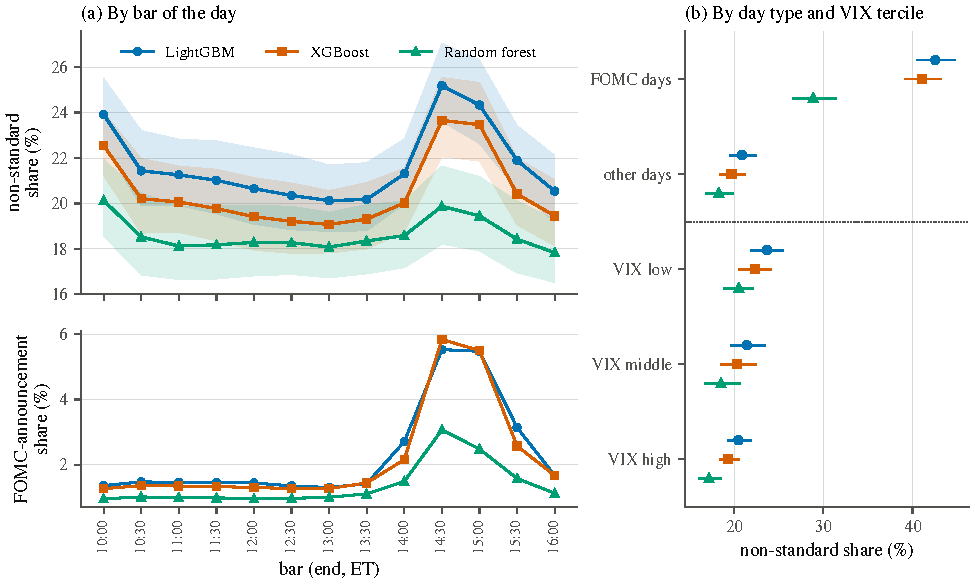
\includegraphics[width=\linewidth]{figures/fi_pooled/fip_cond.pdf}
\caption{When the tree ensembles use the non-standard series. Share of the non-standard series in the total mean absolute SHAP value on subsets of the \rhfipNRows{} bars, with \rhfipCiLevel\% block-bootstrap intervals over the origins. (a) By bar of the day (top; bands: intervals) and the FOMC-announcement category's share (bottom). (b) On the \rhfipFomcDays{} scheduled FOMC statement days and on all other days, and by the tercile of the VIX close before the origin (cut points \rhfipVixLo{} and \rhfipVixHi; every bar of an origin's block takes that origin's tercile).}
\label{fig:rh_fip_cond}
\end{figure}
